\chapter{Methods}
\label{chap:method}

This chapter will cover the specific implementation details of the concepts researched in this thesis. To reiterate, this work systematically investigates the performance of previous state-of-the-art IAD approaches on logical anomalies and interprets the results. Secondly, this paper introduces a feature-level ensemble approach for combining potentially heterogeneous anomaly detection methods to achieve greater robustness. 
These contributions 
are thematized in regards to their execution in the respective sections \ref{sec:lcocsurveymethods} and \ref{sec:ourensemblenetwork} of this chapter. All methods below are 
trained and evaluated on the MVTecAD LOCO dataset and our novel dataset class in chapter \ref{chap:experiments}


\section{Logical Anomaly Detection}
\label{sec:lcocsurveymethods}

As discussed in the introductory chapter \ref{chap:introduction}, logical anomalies represent a significant part of image anomaly detection in modern
manufacturing settings. The experiments also extensively compare state-of-the-art methods for IAD versus recent approaches  
introduced with mind to logical anomalies, like GCAD \cite{LOCODentsAndScratchesBergmann2022}. 
Moreover, for a qualitative evaluation of the performance change when using feature-level ensembles, one first needs to evaluate the base performance 
of each relevant classifier of the set. 
Hence, this work features experiments to evaluate IAD approaches, mainly evaluated on the classical MVTecAD dataset. To do so, the original 
code from each paper was taken and not modified regarding any reported parameters and arguments. This was to prevent unwanted deviations 
in original performance by changing up synergies of hyperparameters. This paper recognizes the possibility of improved performances on the logical anomalies dataset 
with other combinations of model parameters. However, this work focuses on the result assessment of current unmodified approaches and, more importantly, the increased robustness of ensembles. Therefore, research regarding this hypothetical improvement must be done in future work. Metrics specifically looked at in this context are the AUROC, pixel AUROC and the sPRO. 
If the functionality to evaluate these metrics was already given, the inference results were taken from the original code. Otherwise, the according functionality 
was implemented in this work and used to produce the according metrics. Moreover, the results investigate possible causes and effects regarding the segmentation/localization results of the 
classifiers. This is not done according to an official metric but in a more descriptive sense.
Papers whose approaches were evaluated using the MVTecAD LOCO dataset were: SimpleNet \cite{liu2023simplenet}, PatchCore \cite{patchCore2022}, Reverse Distillation \cite{revdist2023} and DRAEM \cite{Zavrtanik_2021DRAEM}. 
These papers were discussed in more depth in the backgrounds section, and any specifics, such as 
hyperparameters, can be viewed in the corresponding paper. Furthermore, all named classifiers included, among other variable measures, 
a preprocessing step to resize the input image. This makes for variable model input and the ability to process rectangular images, 
which is vital due to MVTecAD LOCO images being rectangular, unlike the squared input from the standard MVTecAD dataset. The only 
necessary modification to the whole process of anomaly detection was the generation of image masks. The MVTecAD LOCO dataset stores its 
masks in multiple black and white images, one for each anomaly. To fix errors stemming from this fact, additional 
code was added that pastes all masks belonging to one image into a single mask before iterating through the data. 




\section{Ensemble network}
\label{sec:ourensemblenetwork}

%!BILD von pipeline machen!

The following subsections deal with the individual components of our ensemble network pipeline, referencing concepts discussed in chapter \ref{chap:background}. Our Ensemble pipeline 
consists of multiple parts (Fig. \ref{fig:ensemblepipeline}). Firstly, we leverage different feature representations to act as ensemble members, comprising 
different pretrained feature extractors combined with trained feature adapters. Section \ref{sec:ensemblecandidates} elaborates on the choices of candidate backbones. Next, the pipeline 
utilizes concepts discussed in section \ref{sec:ensembles} to merge the different feature representations into one. Afterwards, we adopt the process of SimpleNet's \cite{liu2023simplenet} 
approach to train a simple two-layer discriminator for differentiating between real features and ones altered by Gaussian noise. Before the merged features are input into the 
discriminator, they are projected by a global feature adapter, trained in parallel to the discriminator. Section \ref{sec:discriminator} further discusses this procedure.

\begin{figure}[htbp]
    \centering
    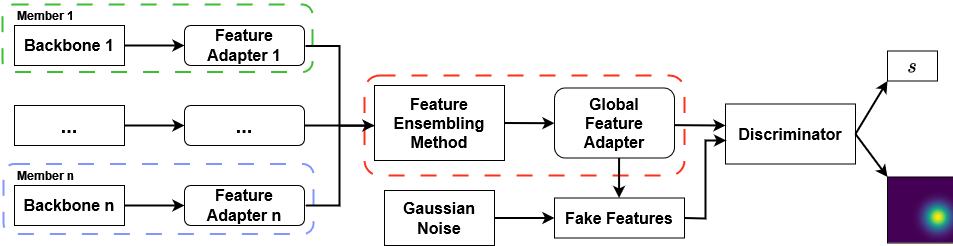
\includegraphics[width=\textwidth]{figures/ensemblepipeline.png}
    \caption{Visualization of the ensemble pipeline. Multiple pairs of feature extractors (backbones) and feature adapters comprise the new backbones of the ensemble. They are 
            merged using any ensembling methods discussed below and then projected by a global feature adapter. Similar to SimpleNet \cite{liu2023simplenet}, the 
            features are then used to generate fake, noisy features and all maps are used as input to train the discriminator.}
    \label{fig:ensemblepipeline}
\end{figure}


\subsection{Ensemble Members}
\label{sec:ensemblecandidates}

We need multiple feature representations to combine for the ensemble to be one. Since the overall ensemble strategy heavily relies on SimpleNets \cite{liu2023simplenet} architecture, 
it is fitting to utilize features derived by separate backbones, along with an according trained feature adapter.\newline
The backbones used are all residual networks by nature: ResNet18 \cite{He_2016resnet}, ResNet50 \cite{He_2016resnet} and Wideresnet50 \cite{wideresnet}. SimpleNet cuts off its 
standard backbone Wideresnet50 at its middle two layers, layer two and layer three, and then aggregates the extracted features. The first ensemble experiment will combine 
feature representations from all three backbones, cut off at the same layers as the standard procedure. Additionally, a second experiment will aggregate features 
from various hierarchies. This is founded on the knowledge that each network hierarchy contains individual feature representations as visualized in Fig. \ref{fig:featurelayers}. 
These images, taken from \cite{openaifeaturerepres}, showcase how features differentiate themselves at distinct levels. Early features often represent simple patterns like edges, 
while ones taken later from a network make up increasingly complex objects and relationships. Therefore, combining several levels of representation could aid in segmenting 
multiple regions of varying textures.

\begin{figure}[htbp]
    \captionsetup[subfigure]{justification=centering}
    \centering
    \begin{subfigure}[b]{0.25\textwidth} % Decreased width to add space
        \centering
        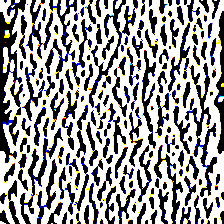
\includegraphics[width=\textwidth]{figures/featurelayersviz/low_channel.png}
        \caption{Lower Level Features}
    \end{subfigure}
    \hspace{0.05\textwidth} % Add space between subfigures
    \begin{subfigure}[b]{0.25\textwidth} % Decreased width to add space
        \centering
        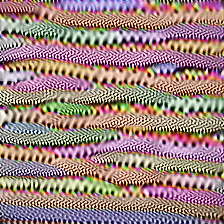
\includegraphics[width=\textwidth]{figures/featurelayersviz/medium_channel.png}
        \caption{Mid Level Features}
    \end{subfigure}
    \hspace{0.05\textwidth} % Add space between subfigures
    \begin{subfigure}[b]{0.25\textwidth} % Decreased width to add space
        \centering
        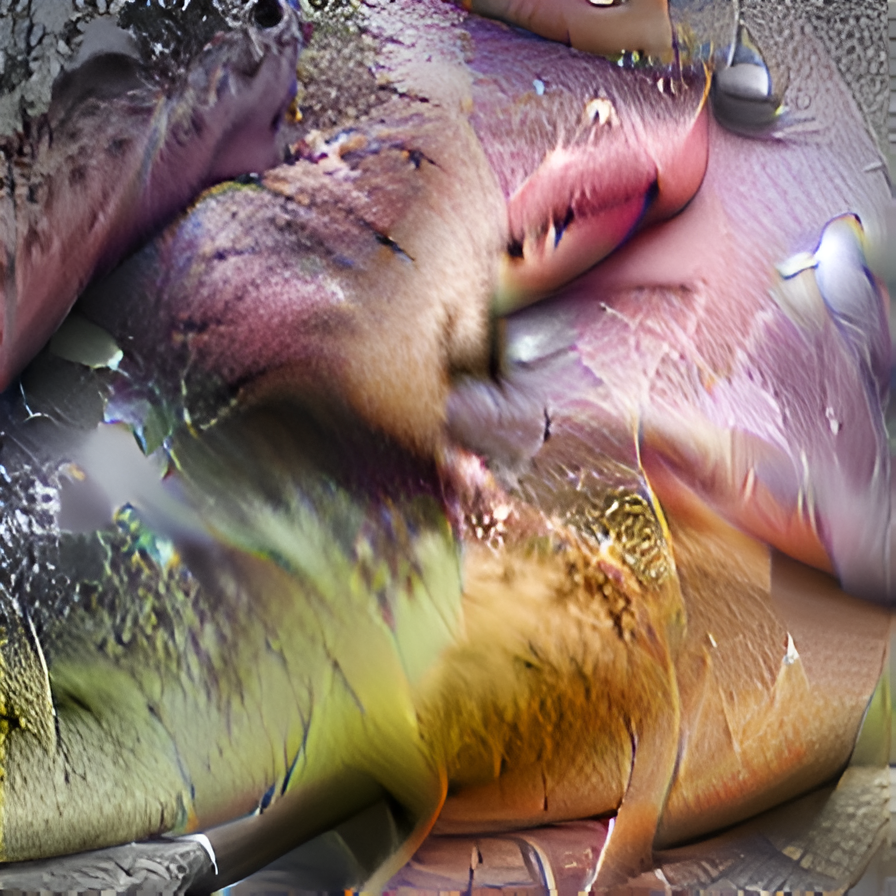
\includegraphics[width=\textwidth]{figures/featurelayersviz/late_channel.png}
        \caption{Higher Level Features}
    \end{subfigure}
    \caption{Illustration of Feature Representations at Different Levels}
    \label{fig:featurelayers}
\end{figure}

One aspect to remember is that the backbones are pretrained and do not necessarily have feature outputs in the same space. 
To solve this problem, we trained a feature adapter from SimpleNet for each of the backbones before assembling the features. 
This ensures that all feature representations are in the same space and can be ensembled appropriately. The resulting feature vectors are also projected with an additional global 
feature adapter that is trained parallel to the ensemble discriminator.


\subsection{Feature Level Ensembling}
\label{sec:featurelevelensemble}

For combining the feature representations from the ensemble members, we chose the approach of the independent transformation block (see Fig. \ref{fig:ITBheller}, section \ref{sec:ensembles}). This means 
PCA was first performed on each set of feature vectors before then resizing and concatenating them. As for resizing, 
the feature vectors were bilinearly interpolated to the largest dimensions of the ensemble candidates. Moreover, the amount of feature maps kept per classifier, namely $\alpha$ in Fig. \ref{fig:ITBheller}, 
was derived by dividing up the number of feature maps from the first classifier in the list of ensemble members, which in this instance also was the maximum amount. If the number 
was not evenly divisible, excess maps would be split up among the remaining classifiers as evenly as possible.\newline
As stated in the results under subsection \ref{subsec:ITBfail} and further analyzed in section \ref{subsec:ITBfaildiscussion}, this approach did not yield the expected results. 
A solution to briefly bridge this problem was to simply stack the channels of the ensemble members' feature maps. This produced the results shown and discussed in the respective 
sections \ref{subsec:stacking} and \ref{subsec:stackingdiscussion}.


\subsection{Ensemble Training}
\label{sec:discriminator}
Our approach to using a small, compact discriminator to differentiate between regular and anomalous image features is based on the concept of 
one-class classification from the representation-based approaches. Specifically, the main inspiration of this work is the approach 
presented in SimpleNet \cite{liu2023simplenet}. Since our discriminator inputs in the ensemble pipeline, which stems from ensembled locally aware patch features, 
will be similar as 
the inputs for SimpleNet's discriminator, it is reasonable to utilize their network architecture for this work. Looking back at section 
\ref{subsec:simplenet} and moreso Fig. \ref{fig:simplenetpipeline}, we thus will adapt the SimpleNet pipeline at the feature adapter step. 
This means we will train a global feature adapter that ensures the projection of ensembled features into the right latent space. Additionally, a lightweight discriminator 
is trained, which again differentiates between normal ensembled features and artificially created abnormal ones. Unlike in the original approach, the input to the feature adapter 
does not consist of only pre-extracted image features 
but the ensembled features from section \ref{sec:featurelevelensemble}. The artificial anomalous features, 
depicted as the red-tiled pane in Fig. \ref{fig:simplenetpipeline}, will also be provided during training time. Here, we also adapt SimpleNet's approach of 
Gaussian noise to produce those artificial features. %(Simplex noise???). 
The discriminator is expected to provide positive and negative outputs for regular and anomalous features, respectively.
As to the discriminator network specifics, a regular fully connected network consisting of two layers is used. As an optimizer, this work utilizes the 
Adam optimizer by Pytorch with a learn rate of 0.0002. The loss is derived the same way as in the approach that inspired this procedure, 
which is according to equation \ref{eq:simplenetloss}.


\subsection{Calibration}
\label{sec:Calibration}

As discussed in section \ref{sec:modelcalibration}, calibration can significantly improve the understanding and usability of classifiers. Anomaly models researched in this work only return non-probabilistic 
outputs. These can be thresholded to derive decision criteria but do not represent any output confidence of the model at all. When looking back at \cite{Guo_2017_tempscalingetc}, the only calibration 
method for binary classifiers that did not need a probabilistic output was the platt scaling attempt. Therefore, this basic principle was the method of choice for calibrating the ensemble network 
outputs. It is to be noted here that we merely calibrate the model's final outputs after everything has been predicted. This stems from the fact that \cite{Wu_2021_shouldbecalibrated} demonstrated 
how calibrated ensemble members do not necessarily yield a well-calibrated final output, shifting our focus to calibration application. During the process, it became apparent that the platt 
scaling approach from \cite{Guo_2017_tempscalingetc} was not necessarily sufficient, as Fig. \ref{fig:badCal} demonstrates. The graph displays 20 predicted scores of the "broken large" anomaly of the bottle class of the MVTecAD dataset, 
along with the predicted anomaly scores of 20 normal images. Notably, the scores were not additionally sorted but naturally 
were linearly separable. The y-axis score of one denotes an anomalous image, and 0 is a normal one.


\begin{figure}[htbp]
    \centering
    \begin{subfigure}[b]{0.45\textwidth}
        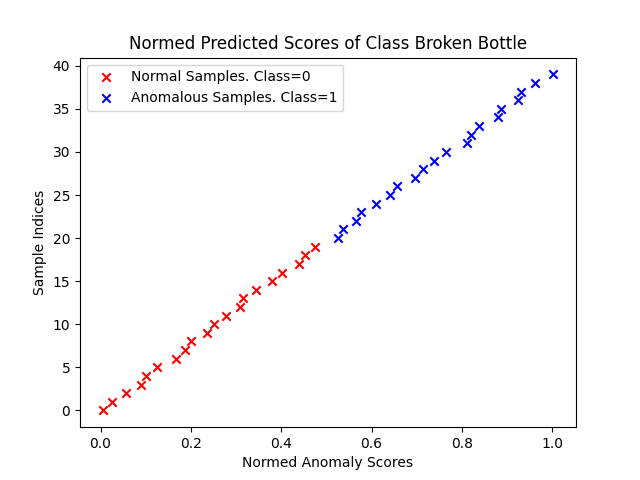
\includegraphics[width=\textwidth]{figures/anomaly_scores_sorted.png}
        \caption{Normed anomaly scores for images of the broken bottle class and normal images.}
        \label{fig:scoresNormed}
    \end{subfigure}
    \begin{subfigure}[b]{0.45\textwidth}
        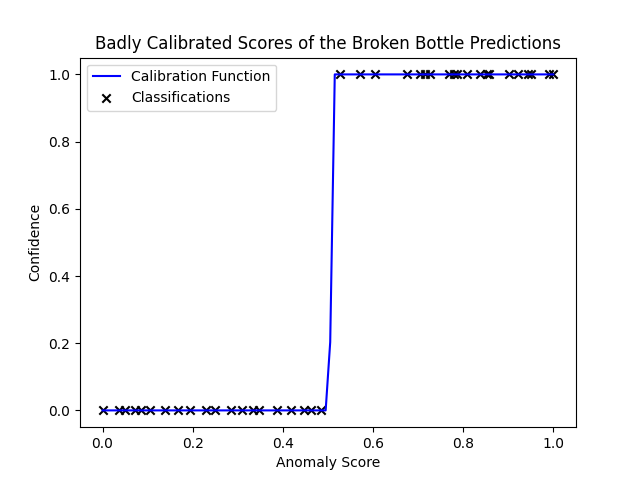
\includegraphics[width=\textwidth]{figures/anomaly_calibration_step.png}
        \caption{Applied platt scaling calibration for the normed scores.}
        \label{fig:platt}
    \end{subfigure}
    \caption{The normed anomaly scores for the MVTecAD \cite{MVTEC_Bergmann_2021} class broken bottle. b) is applied platt scaling calibration. The x-axis represents 
            the anomaly score value for each entry, and the y-axis the confidence for the curve. Here, confidence is defined as the confidence that the sample is anomalous}
    \label{fig:badCal}
\end{figure}

Due to the high performance of some IAD algorithms, some categories 
of the datasets may be entirely correctly classified, which, for example, was the case here. This would mean that the optimal fitted sigmoid curve on the points 
is a step curve, yielding either 100 percent confidence or none at all. This does not seem well calibrated, especially not looking at the exemplary score distribution in Fig. \ref{fig:platt}, where the predicted anomaly scores seem to be stretched pretty evenly over the interval. There is an argument on how a step 
curve would be appropriate for such cases since the model classified each sample correctly and can thus be entirely certain whether an 
image is anomalous. However, this might make data hard to interpret as everything inside one class 
would have the same certainty. For example, a point barely above the threshold would have the same certainty as the point furthest away from it, 
which seems not necessarily appropriate and does not capture any uncertainty variance.
We propose a generalized bounded sigmoid function with a variable slope \cite{bounded_sigmoid} as seen in equation \ref{eq:boundedsigmoid}. This allows the user to calibrate the steepness of the slope to account for larger uncertainty 
towards the decision threshold.

\begin{equation}
    \label{eq:boundedsigmoid}
    \begin{split}
        s_{k, t}(x) = \frac{1}{1 + (x^{\frac{log(2)}{log(t)}} - 1)^{k}}
    \end{split}
\end{equation}

$t$ denotes the point where the function has to pass through. This value is usually assigned the calculated threshold for the decision criterion of the classification task. $k$ is a parameter 
that influences the growth of the curve along the axis. This value can either be chosen by hand or optimized regarding uncertainty requirements. This means that if one generally wants the 
outputs to reflect a higher uncertainty towards the threshold, it is reasonable to choose a lower value for k and vice versa. Fig. \ref{fig:sub1} and Fig. \ref{fig:sub2} demonstrate the effects of changing values for k, as well 
as an exemplary well-calibrated platt scaling variant of Fig. \ref{fig:sub3}, using the presented formula.

\begin{figure}[htbp]
    \centering
    \begin{subfigure}[b]{0.3\textwidth}
        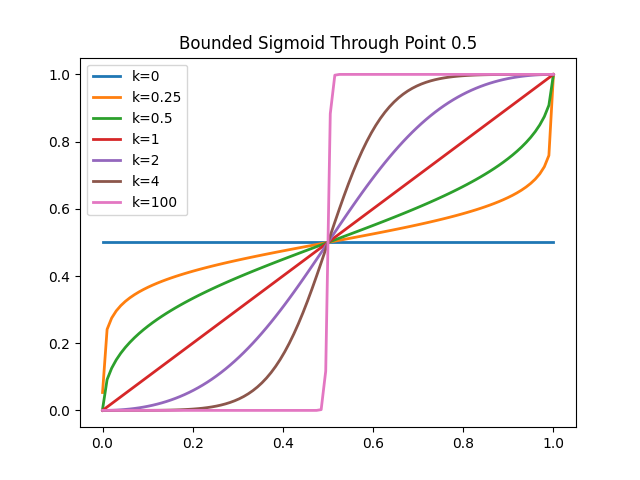
\includegraphics[width=\textwidth]{figures/soft_sigmoidt05.png}
        \caption{Function Values for $t=0.5$ and Various k-Values}
        \label{fig:sub1}
    \end{subfigure}
    \hfill
    \begin{subfigure}[b]{0.3\textwidth}
        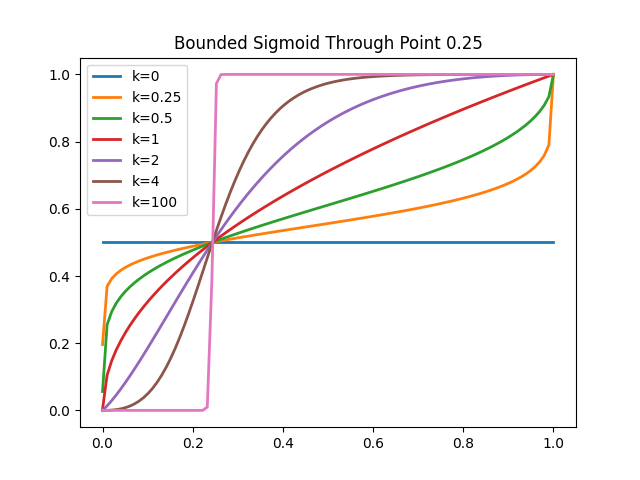
\includegraphics[width=\textwidth]{figures/soft_sigmoidt25.png}
        \caption{Function Values for $t=0.25$ and Various k-Values}
        \label{fig:sub2}
    \end{subfigure}
    \hfill
    \begin{subfigure}[b]{0.3\textwidth}
        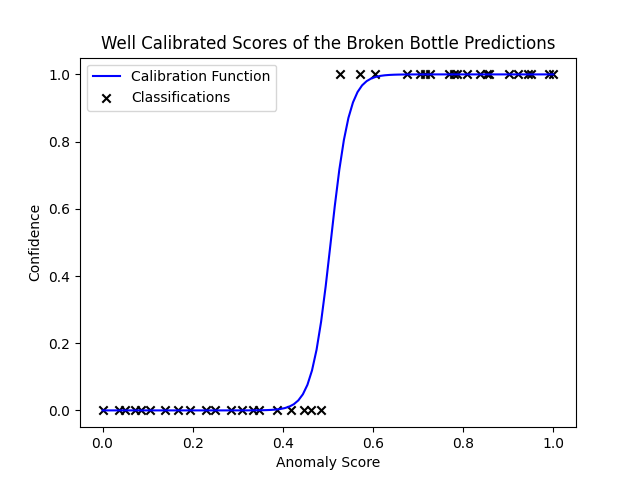
\includegraphics[width=\textwidth]{figures/anomaly_calibration_soft.png}
        \caption{Well Calibrated Scoring Function for Broken Bottle Class}
        \label{fig:sub3}
    \end{subfigure}
    \caption{Effects of changing parameters k and t and exemplary calibration for the MVTecAD \cite{MVTEC_Bergmann_2021} class broken bottle}
    \label{fig:calicalibraction}
\end{figure}

This calibration method is provided in the pipeline to produce an uncertainty metric. Yet, in light of the reported metrics of other IAD research, the experiments and discussion will only 
review the same metrics, namely image and pixel AUROC and the PRO, or rather sPRO, score.








